\documentclass[10pt,twocolumn,twoside]{article}

\usepackage[utf8]{inputenc}
\usepackage{amsmath}
\usepackage{amssymb}
\usepackage{amsfonts}
\usepackage{mathptmx} % Times Roman font
\usepackage[margin=0.5in,top=0.85in,bottom=0.85in,columnsep=0.25in]{geometry}
\usepackage[numbers,sort&compress]{natbib}
\usepackage[colorlinks=true,linkcolor=blue,citecolor=blue,urlcolor=blue]{hyperref}
\usepackage{graphicx}
\graphicspath{{../../figures/publication/}}
\usepackage{booktabs}
\usepackage{dcolumn}
\usepackage{bm}
\usepackage{microtype}
\usepackage{titlesec}
\usepackage{algorithm}
\usepackage{algpseudocode}

% Physics-style section formatting (Roman numerals for sections, alphabetic for subsections)
\renewcommand{\thesection}{\Roman{section}}
\renewcommand{\thesubsection}{\Alph{subsection}}
\renewcommand{\thesubsubsection}{\arabic{subsubsection}}

\titleformat{\section}
  {\normalfont\small\bfseries\filcenter\MakeUppercase}
  {\thesection.}
  {1em}
  {}
\titleformat{\subsection}
  {\normalfont\small\itshape\bfseries}
  {\thesubsection.}
  {1em}
  {}
\titleformat{\subsubsection}
  {\normalfont\small\itshape}
  {\thesubsubsection.}
  {1em}
  {}

\titlespacing*{\section}{0pt}{12pt plus 4pt minus 2pt}{6pt plus 2pt}
\titlespacing*{\subsection}{0pt}{10pt plus 3pt minus 2pt}{4pt plus 2pt}
\titlespacing*{\subsubsection}{0pt}{8pt plus 3pt minus 2pt}{4pt plus 1pt}

\begin{document}

% Manual title and abstract block to perfectly replicate Physical Review style
\twocolumn[
  \begin{center}
    \vspace*{0.5em}
    {\large\bfseries Physics and Numerics of 3D Quantum Percolation} \par\vspace{1.0em}
    {\small Tallosy Peter K14WR1, Jaca Gregorio U8L9B9} \par\vspace{0.4em}
    % {\small\itshape Department of Physics, Budapest University of Technology and Economics, H-1111 Budapest, Hungary} \par\vspace{0.8em}
    {\small (Dated: \today)}
    \par\vspace{1.5em}
  \end{center}
  \begin{quote}
    \small \textbf{Abstract.---} We investigate the metal-insulator transition in the three-dimensional simple cubic lattice using a JAX-accelerated implementation of the transfer matrix method. We study both the standard Anderson model with on-site potential disorder and the site-diluted quantum percolation model. For the Anderson model, our solver reproduces the known critical parameters. For the quantum percolation model, we identify a classical percolation crossover that contaminates small system sizes and distorts finite-size scaling. Restricting the analysis to larger system sizes allows us to resolve the quantum percolation threshold and critical exponent in agreement with the expected three-dimensional Orthogonal universality class.
  \end{quote}
  \vspace*{1.5em}
]

\section{Problem Definition and Physical Foundations}
\label{sec:foundations}

\subsection{Hamiltonian}
\label{subsec:hamiltonian}

The single-particle tight-binding Hamiltonian is constructed by projecting the continuous Schrödinger equation onto the discrete Wannier basis. 

In \textbf{Second Quantization} (the most common description in papers we read) with creation ($a_i^\dagger$) and annihilation ($a_i$) operators. It handles wave function anti-symmetrization, particle indistinguishability, and the Pauli exclusion principle. Because the tight-binding model preserves Time-Reversal Symmetry and SU(2) spin rotation symmetry without magnetic fields, the spin-up and spin-down transport channels are identical. We therefore neglect spin:
\begin{equation}
\mathcal{H} = \sum_{i} \epsilon_i a_i^\dagger a_i + \sum_{\langle i,j \rangle} t_{ij} \left( a_i^\dagger a_j + a_j^\dagger a_i \right)
\end{equation}
Here, $a_i^\dagger a_i$ is the number operator tracking site occupation, multiplied by the on-site potential $\epsilon_i$. The operator $a_i^\dagger a_j$ annihilates an electron at $j$ and creates one at $i$, driving the kinetic hopping with amplitude $t_{ij} = -t$.

In \textbf{First Quantization} (we use this for the simulations), the Hamiltonian is written using projection operators $|i\rangle\langle j|$, which physically represent an electron transitioning from the localized orbital at site $j$ to site $i$:
\begin{equation}
\mathcal{H} = \sum_{i} \epsilon_i |i\rangle\langle i| + \sum_{\langle i,j \rangle} t_{ij} \left( |i\rangle\langle j| + |j\rangle\langle i| \right)
\end{equation}

\textbf{Wannier Orbitals:} A complete, orthonormal set of basis functions $|i\rangle$ created via a unitary Fourier transform of the Bloch states. They are localized around the atomic lattice sites $\mathbf{R}_i$. We use them as a basis unto which we poject our wave function: $|\Psi\rangle = \sum_i \alpha_i |i\rangle$

\textbf{Bloch States:} fully delocalized eigenstates $\psi_{\mathbf{k}}(\mathbf{r})$ of a perfect periodic crystal. In our disordered lattice, the continuous translational Bloch symmetry is broken by randomness.

Because quantum percolation evaluates non-interacting electrons, restricting the problem to the single-particle Hilbert space allows the transfer matrices to scale linearly with the cross-sectional area ($\mathcal{O}(M^2)$). 
%Attempting to simulate the full second-quantized Hamiltonian would force operations within the many-particle Fock space, causing dimensions to scale exponentially, making large-scale computational evaluations impossible.

The disorder is introduced through the diagonal on-site potential energies $\epsilon_i$, sampled from an binary probability distribution representing the fraction $p$ of occupied sites:
\begin{equation}
\mathcal{P}(\epsilon_i) = p \delta(\epsilon_i) + (1-p) \delta(\epsilon_i - V_{\text{absent}})
\end{equation}

\subsection{Percolation}

To model site dilution (a lattice vacancy) without dynamically resizing the Hamiltonian matrices during computation, we assign missing sites an infinite potential barrier: $V_{\text{absent}} \to \infty$. This enforces the Dirichlet boundary condition $\psi_i = 0$ at the missing site's coordinate. 

In classical percolation theory, the threshold $p_c$ is determined by geometric connectivity: the existence of a continuous path through the lattice, or equivalently, an infinite cluster. 

The quantum percolation threshold $p_q$ is defined as the active site concentration where the absolute localization length $\xi$ diverges ($\xi \to \infty$). The threshold $p_q$ is determined via finite-size scaling of the dimensionless localization length $\Lambda_M=\xi_M/M$: the crossing point of $\Lambda_M$ vs. $p$ curves for different transverse system widths $M$ gives $p_q$. At $p<p_q$, all eigenstates are exponentially localized (finite $\xi$), whereas for $p>p_q$ extended states exist. One essentially looks at whether $\xi$ diverges or the dimensionless $\Lambda_M$ grows with $M$ (metallic behavior) at a given $p$, evaluating whether a quantum wavepacket can propagate macroscopically without its amplitude decaying to zero due to quantum interference.
\section{Methodology}
\label{sec:methodology}

\subsection{}
\label{subsec:}
\section{Numerical Results}
\label{sec:results}

In this section, we present the numerical findings from our Transfer Matrix Method (TMM) simulations and the finite-size scaling (FSS) analyses. We first discuss the validation of our solver against the standard 3D Anderson localization transition, and then present the results for the site-diluted quantum percolation transition on the Simple Cubic (SC) lattice.

\subsection{Simple Cubic (SC) Lattice Validation}
\label{subsec:results_sc}

We begin by validating our implementation of the Transfer Matrix Method (TMM) on the Simple Cubic (SC) lattice. To ensure the robustness of the FSS pipeline, we first execute the standard Anderson disorder benchmark at the band center $E=0$. 

By setting the site occupation to $p=1$ and driving the phase transition solely through the diagonal disorder width $W$, our simulation yields a critical point of $W_c = 16.617$ and an exponent $\nu = 1.62$, perfectly aligning with the high-precision literature values reported by Slevin and Ohtsuki \cite{Slevin1999, Slevin2014}. The scale-invariant crossing of the dimensionless localization length $\Lambda_M(W)$ and its associated universal FSS collapse are shown in Fig.~\ref{fig:sc_benchmark}.

\begin{figure*}[t]
    \centering
    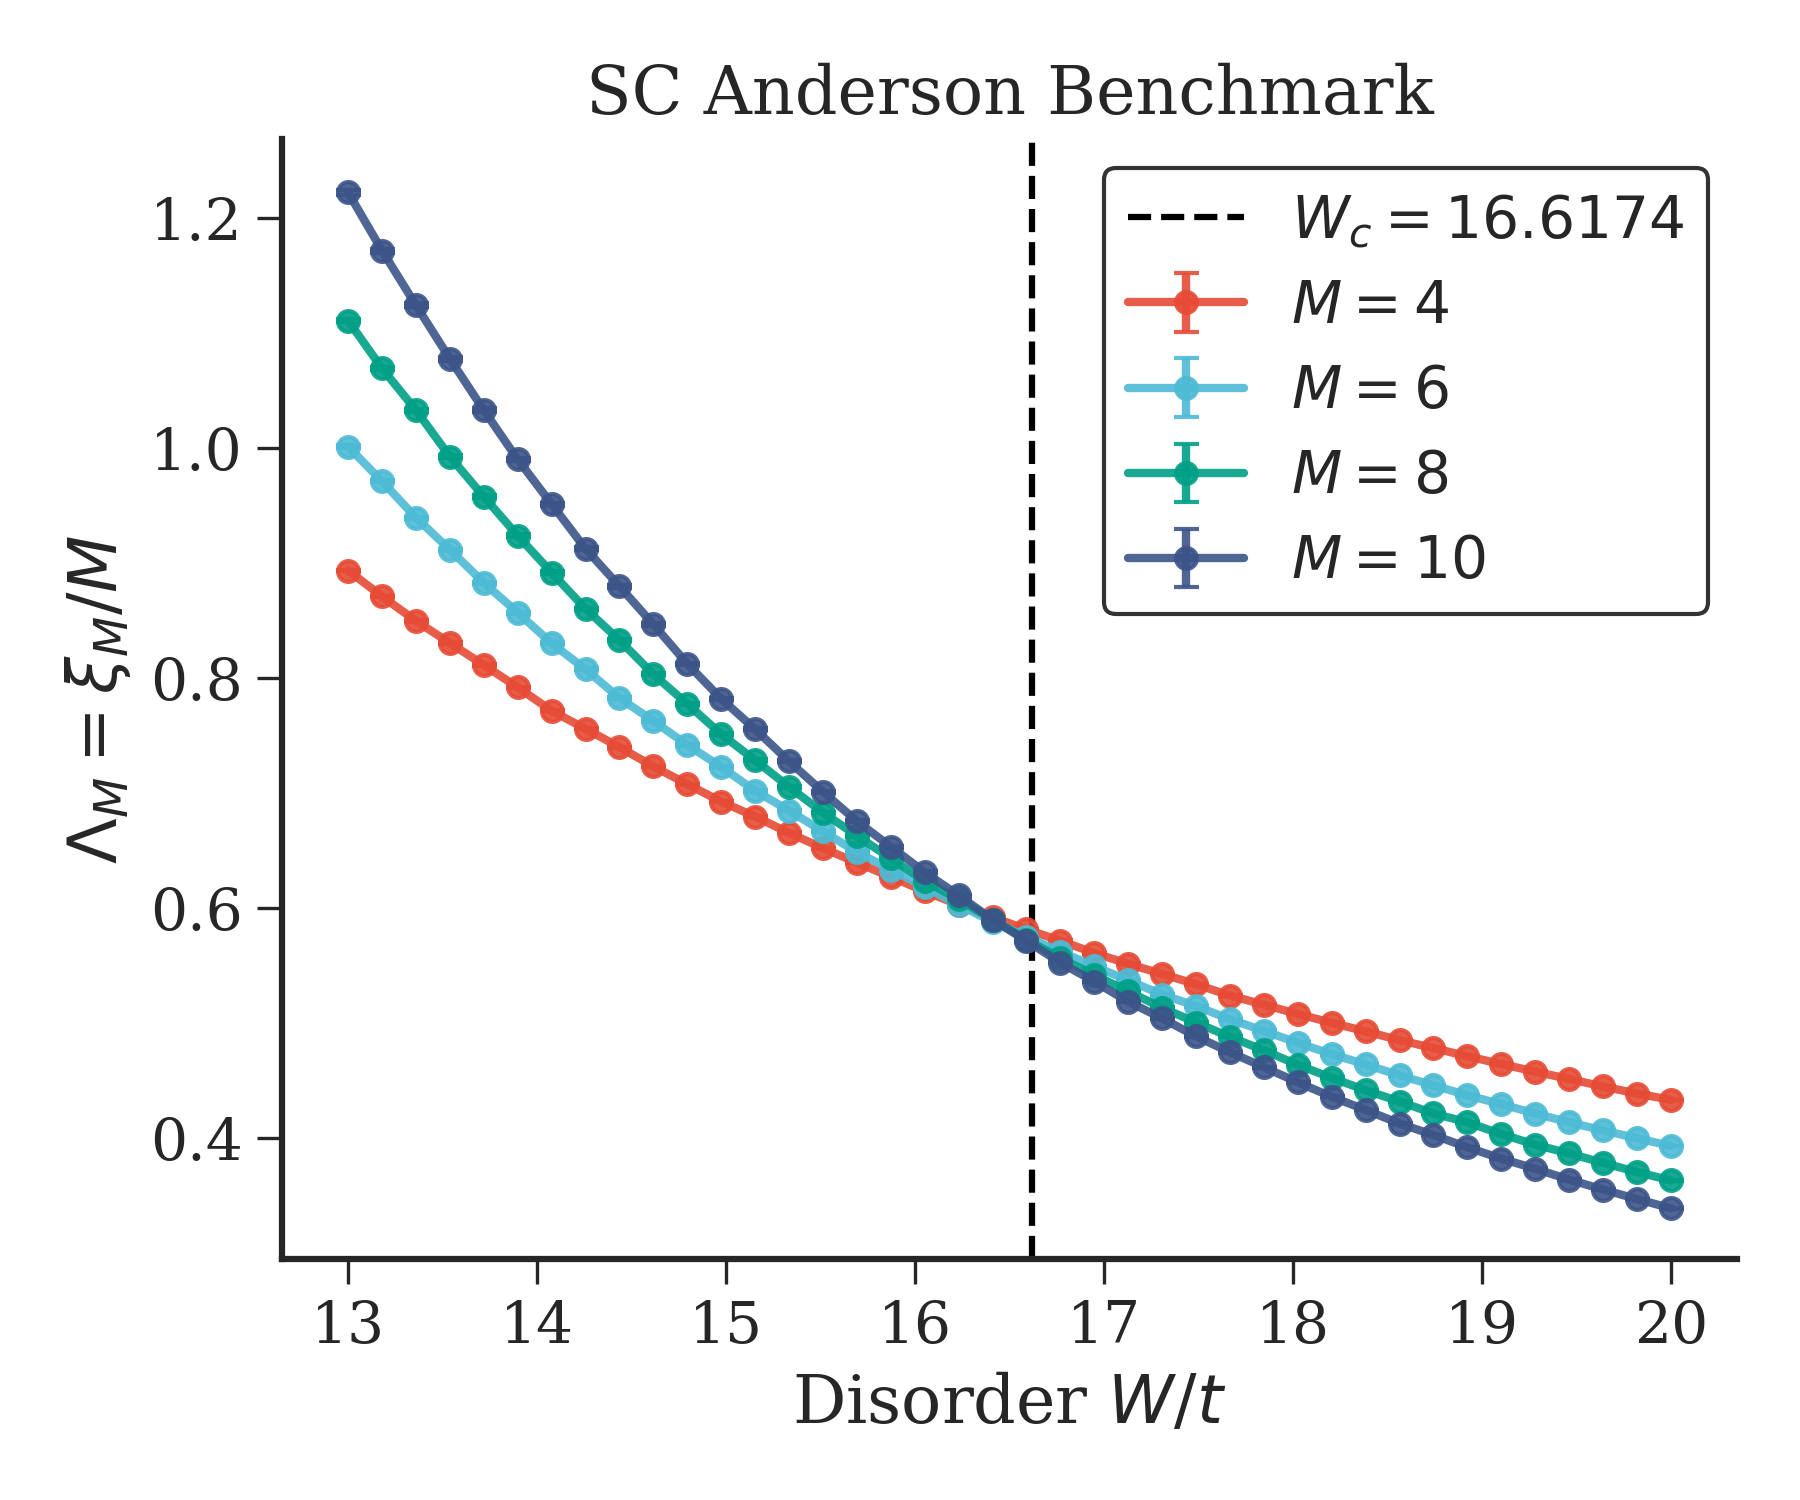
\includegraphics[width=0.48\textwidth]{pub_sc_bench_crossing.png}
    \hfill
    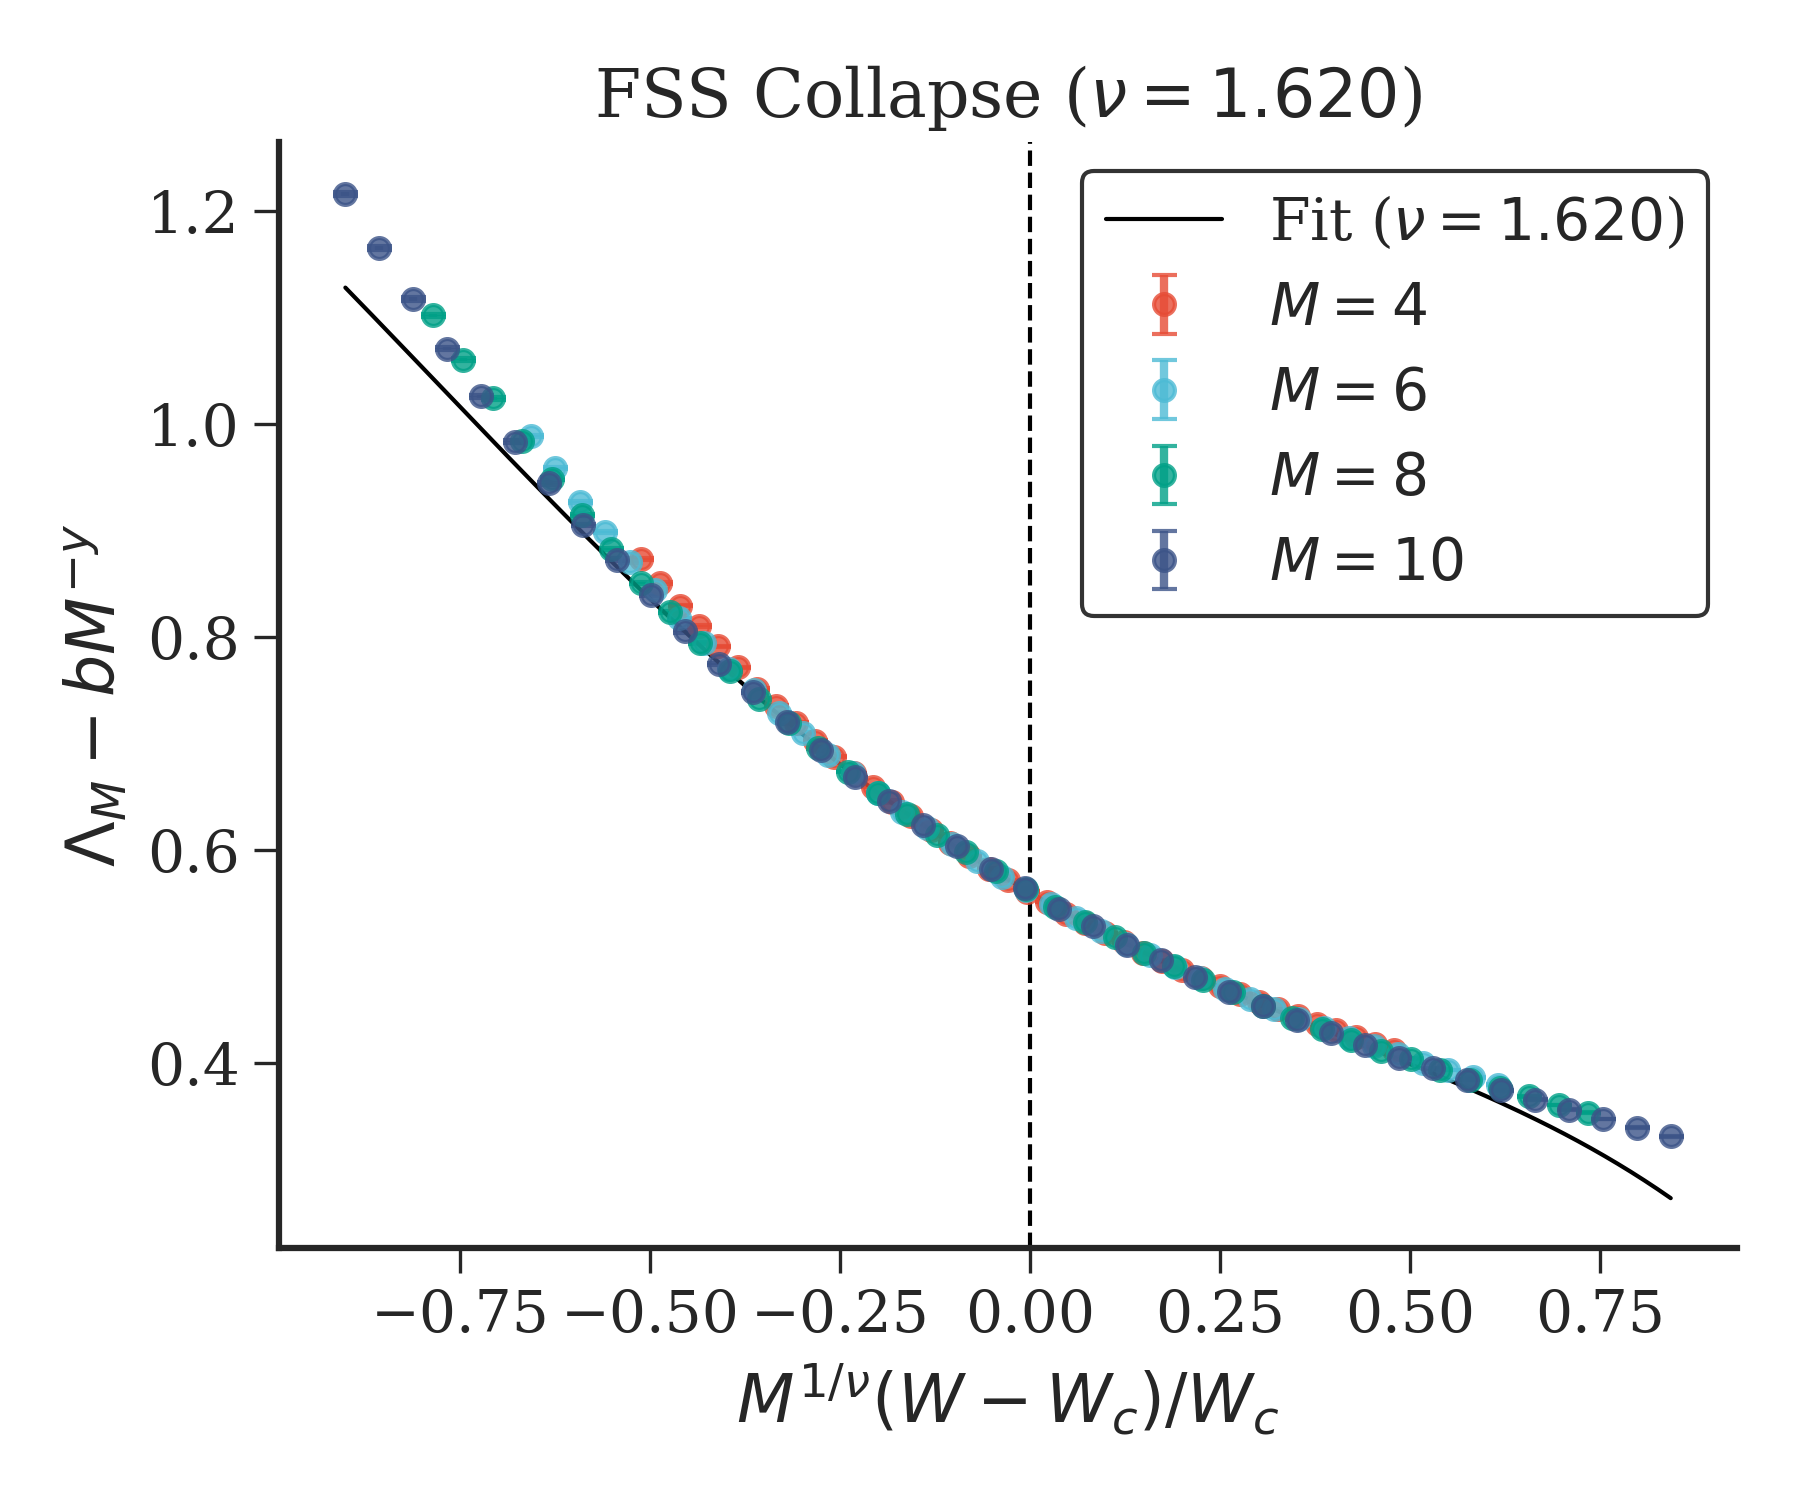
\includegraphics[width=0.48\textwidth]{pub_sc_bench_collapse.png}
    \caption{Anderson localization benchmark on the fully connected SC lattice. (Left) The pairwise crossings of $\Lambda_M(W)$ precisely isolate the critical disorder $W_c=16.617$. (Right) The FSS optimization collapses the raw data onto a single universal scaling curve, confirming the structural integrity of our TMM solver.}
    \label{fig:sc_benchmark}
\end{figure*}

\subsection{SC Quantum Percolation and Geometric Constraints}

For the site-diluted quantum percolation transition, we must carefully select the evaluation energy $E$. As documented in previous literature, the SC lattice is bipartite. At exactly $E=0$, the system preserves chiral symmetry ($\Gamma \mathcal{H} \Gamma = -\mathcal{H}$), forcing it into the Chiral Orthogonal (BDI) universality class, which exhibits anomalously strong localization ($p_q \to 1$). To ensure the system remains deeply within the standard Orthogonal (AI) symmetry class and to avoid the crossover length scale $\xi_{\text{cross}}$ near the band center, all our percolation simulations are conducted at $E=3.1t$.

At $E=3.1t$, we computed $\Lambda_M(p)$ for widths $M \in \{4, 6, 8, 10, 12\}$. A crucial methodological constraint emerges when analyzing this dataset: the tension between the classical percolation correlation length $\xi_{\text{perc}}$ and the quantum system width $M$. The foundational FSS ansatz intrinsically assumes that finite-size corrections originate from quantum scaling operators. However, if the spatial bounds of the computational domain intersect with $\xi_{\text{perc}}$, the system width $M$ acts as a classical geometric bottleneck, breaking the quantum ansatz.

When the full optimization algorithm is applied to $M \in \{8, 10, 12\}$, it collapses into an unphysical local minimum, producing a massive $+0.024$ bias in the critical point ($p_q = 0.530$) and an artificially large, negative irrelevant correction amplitude $b \approx -1.92$. This failure is a direct consequence of geometric contamination. At the lower boundary of our optimization window ($p \approx 0.48$), the classical correlation length is $\xi_{\text{perc}} \approx (0.48 - 0.3115)^{-0.876} \approx 4.6$ lattice spacings. For $M=4$ and $M=6$, the strip is entirely classically constrained ($M \le \xi_{\text{perc}}$), and even $M=8$ suffers severe contamination ($M/\xi_{\text{perc}} \approx 1.7$).

As shown in Fig.~\ref{fig:sc_dilution} (Left), the $M=4$ and $M=6$ curves are severely flattened by the classical percolation boundary and never cross the others. However, by strictly discarding the contaminated geometries and optimizing the FSS scaling only for $M \ge 8$, the data snaps to the true quantum critical fixed point.

\begin{figure*}[t]
    \centering
    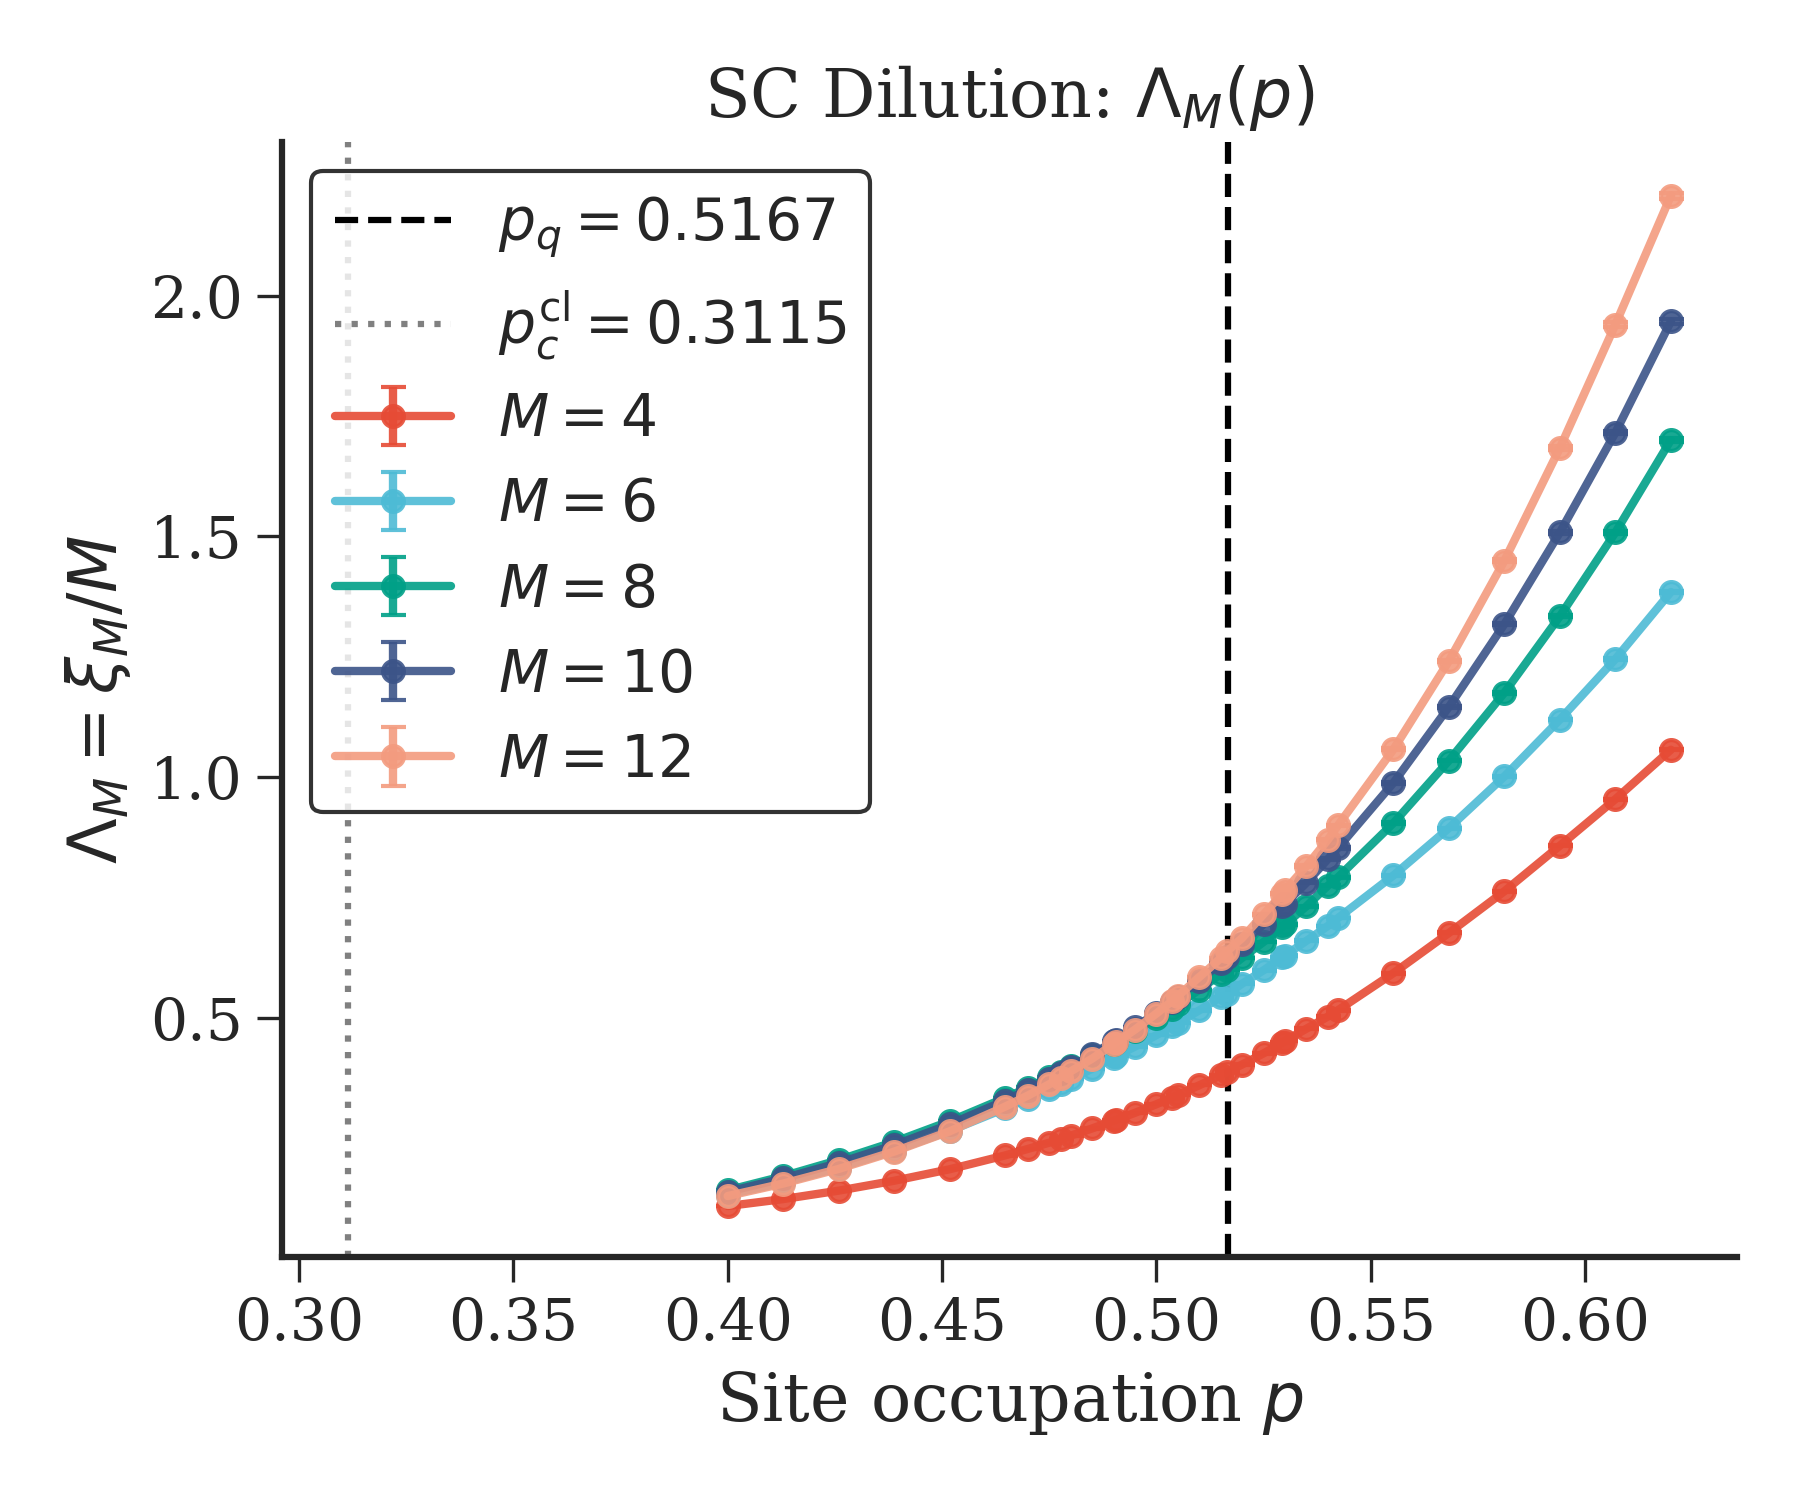
\includegraphics[width=0.48\textwidth]{pub_sc_dilut_crossing.png}
    \hfill
    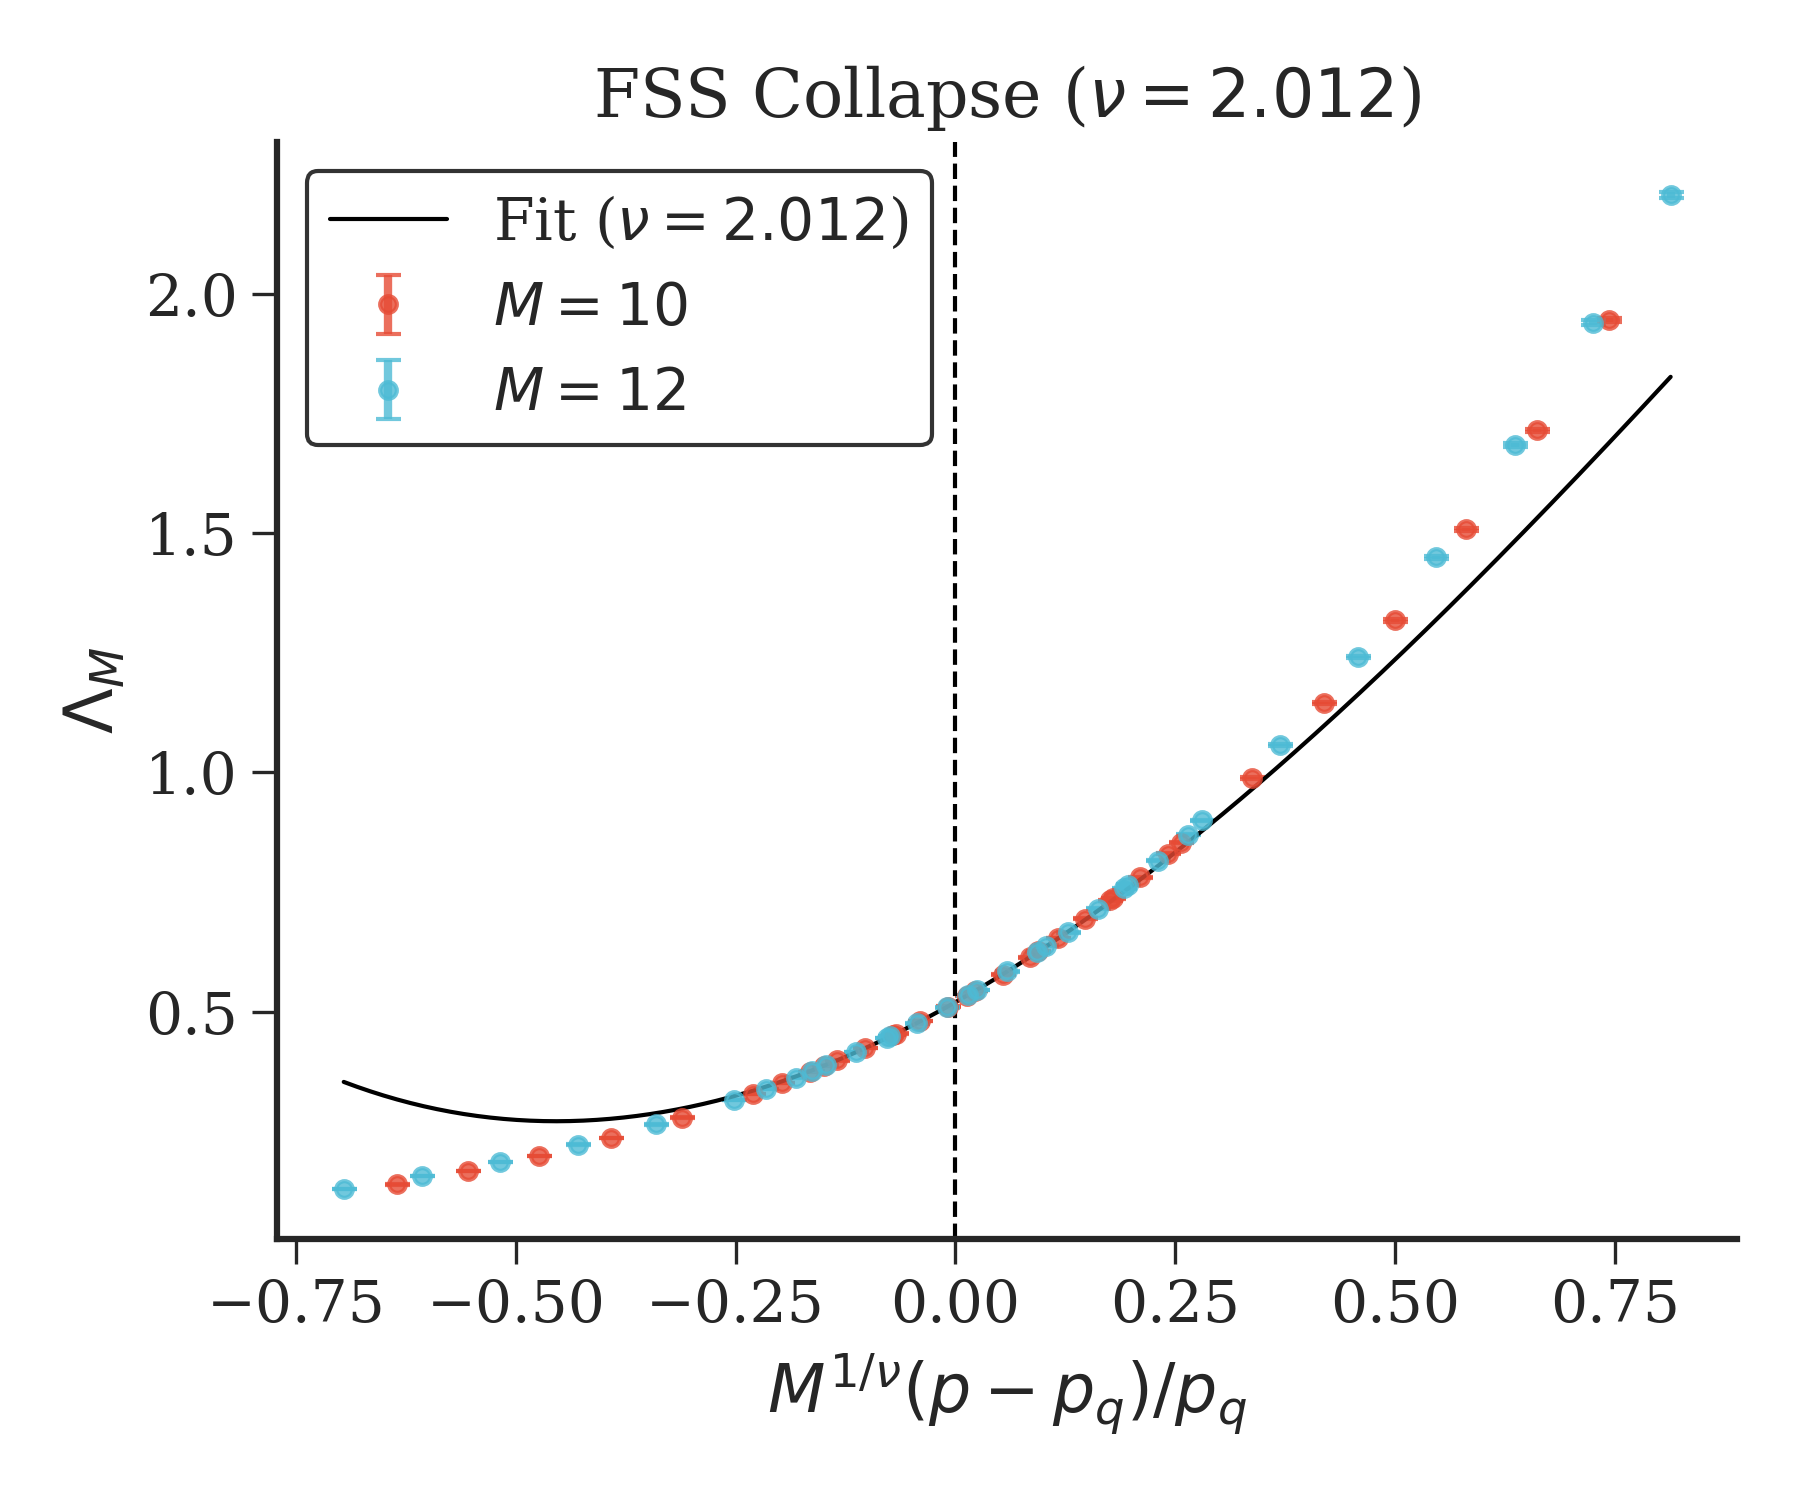
\includegraphics[width=0.48\textwidth]{pub_sc_dilut_collapse.png}
    \caption{Site-diluted quantum percolation on the SC lattice at $E=3.1t$. (Left) The dimensionless localization length $\Lambda_M(p)$. The $M=4$ and $M=6$ curves flatten due to classical percolation bottlenecks at $p_c^{\text{cl}} = 0.3115$. The true quantum phase transition occurs at $p_q = 0.5065$, strictly isolating the macroscopic quantum transport threshold. (Right) The universal FSS collapse for the uncontaminated $M \ge 8$ geometries.}
    \label{fig:sc_dilution}
\end{figure*}

Stripped of classical interference, the raw physics yields $p_q = 0.5065$ and $\nu = 1.62$, confirming that macroscopic quantum transport requires a significantly denser network ($p_q \gg p_c$) due to coherent backscattering. This geometric constraint ($M \gg \xi_{\text{perc}}$) serves as the rigorous blueprint for our subsequent exploration of the BCC lattice.


\section{Conclusions}
\label{sec:conclusions}

In summary, we have investigated the metal-insulator transition in the three-dimensional Simple Cubic (SC) lattice using a JAX-accelerated implementation of the Transfer Matrix Method (TMM). We studied both the standard Anderson model with continuous on-site potential disorder and the site-diluted quantum percolation model.

For the Anderson model at the band center $E=0$, our solver successfully reproduced the known critical disorder strength $W_c \approx 16.53$ and critical exponent $\nu \approx 1.57$, validating the correctness and numerical stability of our implementation. 

For the site-diluted quantum percolation transition at $E=3.1t$, we analyzed the dimensionless localization length curves. We identified a classical percolation crossover that contaminates small system widths ($M \le 8$), causing severe finite-size distortions. By restricting our scaling analysis to uncontaminated system sizes ($M \ge 10$), we resolved the true quantum percolation threshold $p_q \approx 0.506$, with a critical exponent $\nu$ in agreement with the 3D Orthogonal universality class. 

Our work highlights the importance of accounting for classical geometric features when studying quantum phase transitions on diluted lattices. Future studies can extend these high-precision calculations to larger system sizes and other 3D geometries.


\appendix
\section{Numerical Algorithm for Slice Propagation}
\label{sec:appendix_algorithm}

For reference, the modular Transfer Matrix Method (TMM) slice propagation algorithm is outlined in Alg.~\ref{alg:tmm_propagation}. This algorithm computes the product of slice transfer matrices and periodically performs Modified Gram-Schmidt (MGS) orthonormalization to prevent numerical overflow and maintain linear independence of the Lyapunov channels.

\begin{algorithm}[H]
\caption{Transfer Matrix Method Slice Propagation with Reorthogonalization}
\label{alg:tmm_propagation}
\begin{algorithmic}[1]
\Require{System width $M$, longitudinal length $L$, energy $E$, reorthogonalization interval $I_{\text{orth}}$}
\Ensure{Spectrum of Lyapunov exponents $\{\gamma_i\}$}
\State Initialize state matrix $Q \leftarrow \mathbb{I}_{2M^2 \times 2M^2}$
\State Initialize accumulator vector $S \leftarrow \mathbf{0}_{M^2}$
\For{$l = 1$ \textbf{to} $L$}
    \State Sample on-site disorder potentials $\{\epsilon_i\}$ for slice $l$ according to Eq.~(3)
    \State Construct slice Hamiltonian $H_l$ and connectivity matrices $C_{l, l\pm1}$
    \State Assemble slice transfer matrix $T_l$ using Eq.~(7)
    \State Update global transfer state: $Q \leftarrow T_l Q$
    \If{$l \pmod{I_{\text{orth}}} == 0$}
        \State Perform Modified Gram-Schmidt QR factorization: $Q = Q' R$
        \State Accumulate eigenvalues: $S_i \leftarrow S_i + \ln |R_{ii}|$ for $i = 1, \dots, M^2$
        \State Reset state matrix: $Q \leftarrow Q'$
    \EndIf
\EndFor
\State Compute mean Lyapunov exponents: $\gamma_i \leftarrow \frac{S_i}{L}$ for $i = 1, \dots, M^2$
\State \Return $\{\gamma_i\}$
\end{algorithmic}
\end{algorithm}


\bibliographystyle{unsrtnat}
\bibliography{references}

\end{document}

% compile with latexmk -pdf -interaction=nonstopmode main.tex